% Asal-usul (tidak pernah dicetak): lihat sources/outline_sources.md (Tahun 1: morfologi,
% gravitasi, aliran panas dan kegempaan zona subduksi; margin akresi dan erosi; geometri slab;
% busur gunung api). Peta, penampang dan angka Kuril dari figdata/bachelor-1/slab_seismicity.py;
% nilai soal latihan dan soal dihitung dalam kalkulator skrap Buku 3 calc/ch14.py.
\chapter{Margin aktif}\label{ch:b1:active-margins}

Pada 11 Maret 2011, pukul 14.46 waktu setempat, batas lempeng di lepas timur laut Jepang pecah sepanjang sekitar \qty{400}{km} di sepanjang palung dan \qty{150}{km} ke bawah \omterm{def:b1:geological-maps:attitude}{kemiringannya}. Sesar itu tergelincir hingga sebesar 50 hingga \qty{60}{m}, sebagian besar ke arah \omterm{def:b1:geological-maps:attitude}{atas-kemiringan} dari hiposenter, menuju Palung Jepang; di darat, pantai bergeser secara horizontal dan turun. Lempeng yang menunjam di sana, Lempeng Pasifik, masuk ke bawah Jepang sepanjang bidang yang digambarkan oleh gempa bumi hingga ratusan kilometer ke bawah; dan di tempat bidang itu berada sekitar seratus kilometer dalamnya, sederet gunung api berjalan sejajar dengan pantai. Bab ini membaca margin semacam itu dari bentuknya, gravitasinya, \omterm{def:b1:heat-budget:heat-flow}{aliran panasnya} dan, di atas semuanya, gempa buminya.
% ledger: usgs:tohoku, wada:decoupling

\begin{recall}
\omterm{def:b1:layered-earth:lithosphere}{Litosfer} samudra kembali masuk ke dalam \omterm{def:b1:layered-earth:layers}{mantel} di zona subduksi, yang ditandai oleh palung dan zona gempa bumi miring, dan \omterm{def:b1:layered-earth:lithosphere}{litosfer} tua tenggelam di bawah beratnya sendiri (Buku 2, kelas 11); air dari lempeng yang menunjam menurunkan suhu peleburan \omterm{def:b1:layered-earth:layers}{mantel} di atasnya (Buku 2, kelas 12). Panas berdifusi sepanjang jarak $L$ dalam waktu berorde $L^2/\kappa$ (\cref{ch:b1:heat-budget}); slab tak hingga dengan massa jenis $\rho$ dan tebal $h$ menarik dengan $2\pi G\rho h$ (\cref{ch:b1:isostasy-gravity}), lempeng bergerak mengelilingi \omterm{def:b1:plate-kinematics:euler-pole}{kutub Euler} (\cref{ch:b1:plate-kinematics}); \omterm{def:b1:heat-budget:heat-flow}{aliran panas} dasar samudra menurun sebagai akar kuadrat terbalik dari umurnya (\cref{ch:b1:rifts-ridges-margins}).
\end{recall}

\section{Anatomi margin aktif}\label{sec:b1:active-margins:anatomy}

\begin{definition}[Margin aktif, palung samudra, forearc, cekungan busur-belakang]\label{def:b1:active-margins:active-margin}
Sebuah \emph{margin aktif}\index{margin aktif} adalah batas lempeng konvergen tempat \omterm{def:b1:layered-earth:lithosphere}{litosfer} samudra tenggelam di bawah lempeng lain, baik di bawah benua maupun di bawah lempeng samudra lain. Sebuah \emph{palung samudra}\index{palung samudra} adalah lekukan dasar laut yang panjang, sempit dan berbentuk-V, tempat lempeng yang menunjam membengkok ke bawah di bawah yang lain. \emph{Forearc}\index{forearc} adalah bagian dari lempeng yang menindih di antara palung dan deretan gunung api. Sebuah \emph{cekungan busur-belakang}\index{cekungan busur-belakang} adalah cekungan di belakang gunung api, di sisi yang menjauhi palung, tempat lempeng yang menindih teregang dan \omterm{def:b1:rifts-ridges-margins:oceanic-crust}{kerak samudra} baru mungkin terbentuk.
\end{definition}

Palung adalah tempat terdalam di samudra, dan yang terdalam dari semuanya adalah Challenger Deep di Palung Mariana. Melintasi Palung Kuril, dasar turun dari sekitar \qty{5200}{m} di dataran abisal hingga \qty{8700}{m} di sumbunya, sekitar \qty{3.5}{km} lebih rendah, dan palung itu hanya selebar puluhan kilometer (gambar di \cref{sec:b1:active-margins:gravity-heat}). Margin konvergen Bumi berukuran sekitar \qty{55000}{km} seluruhnya; dalam model digital batas-batas lempeng, batas subduksi berjumlah sekitar \qty{51000}{km}, dibandingkan dengan sekitar \qty{67000}{km} punggungan penyebaran.
% ledger: data:b3-grav-kuril (trench_gravity.py values), stern:subduction, data:pb2002 (ridge_budget.py)

Di sisi laut palung, lempeng naik sedikit sebelum menunjam, dalam tonjolan luar yang luas dan rendah. Di sana lempeng membengkok, dan bagian atasnya teregang: gempa bumi sesar normal melanda tonjolan luar. Lebar tonjolan luar sesuai dengan pembengkokan lempeng elastik; lenturan \omterm{def:b1:layered-earth:lithosphere}{litosfer} ini dipelajari dalam Buku 5. Palung sendiri adalah tempat berat lempeng padat yang menunjam menarik tepi depannya ke bawah.

\begin{definition}[Slab yang menunjam]\label{def:b1:active-margins:slab}
\emph{Slab yang menunjam}\index{slab yang menunjam} adalah bagian dari lempeng yang menunjam yang sudah masuk ke dalam \omterm{def:b1:layered-earth:layers}{mantel}: lembaran \omterm{def:b1:layered-earth:lithosphere}{litosfer} samudra, dengan \omterm{def:b1:layered-earth:layers}{kerak} di atasnya, miring di bawah lempeng yang menindih dari palung hingga kedalaman beberapa ratus kilometer.
\end{definition}

Lempeng yang menindih terpotong menjadi jalur-jalur sejajar palung (gambar di bawah): \omterm{def:b1:active-margins:active-margin}{forearc}, sering dengan tumpukan sedimen yang terkikis di bagian depannya dan cekungan sedimen di belakangnya; \omterm{def:b1:active-margins:volcanic-arc}{busur gunung api}; dan, di belakang sebagian busur, \omterm{def:b1:active-margins:active-margin}{cekungan busur-belakang} dan busur tua yang telah punah di belakangnya. Di antara slab dan lempeng yang menindih terdapat baji \omterm{def:b1:layered-earth:layers}{mantel}, terseret ke bawah sepanjang bagian atas slab.

\begin{omfigure}
\begin{tikzpicture}[x=0.01667cm, y=0.01667cm, font=\scriptsize,
  lbl/.style={fill=white, fill opacity=0.8, text opacity=1, inner sep=1pt}]
\begin{scope}
\clip (-150,-330) rectangle (650,55);
% mantle and sea water
\fill[orange!12] (-150,-330) rectangle (650,15);
\fill[omSea!45] (-150,15) rectangle (650,0);
% incoming plate and slab: top dips 25 deg to 50 km, then 45 deg; 100 km thick
\fill[omLithBasalt!55] (-150,4) -- (-80,4) .. controls (-60,7) and (-40,7) .. (-25,4) -- (0,0)
  -- (107.2,-50) -- (420,-363) -- (349,-434) -- (48.9,-133.1) -- (-22.1,-100) -- (-150,-100) -- cycle;
\draw[omSea!50!black, line width=1.6pt] (-150,4) -- (-80,4) .. controls (-60,7) and (-40,7) .. (-25,4) -- (0,0) -- (107.2,-50) -- (420,-363);
% overriding plate
\fill[brown!28] (0,0) -- (12,3) -- (45,8) -- (60,10) -- (140,10) -- (150,12) -- (184,12) -- (230,9)
  -- (300,7) -- (395,6) -- (410,3) -- (420,2) -- (430,3) -- (445,6) -- (540,7) -- (560,14) -- (590,14)
  -- (610,10) -- (650,10) -- (650,-60) -- (520,-55) -- (445,-25) -- (420,-15) -- (395,-25) -- (320,-55)
  -- (250,-60) -- (117.2,-60) -- (107.2,-50) -- cycle;
% accretionary prism and forearc basin
\fill[yellow!55] (0,0) -- (12,3) -- (45,8) -- (60,10) -- (60,-28) -- cycle;
\draw[black!45, line width=0.3pt] (14,-3) -- (24,5) (28,-7) -- (38,6) (42,-14) -- (52,8);
\fill[yellow!30] (68,10) -- (132,10) -- (122,4) -- (78,4) -- cycle;
% arc volcano
\fill[black!60] (150,12) -- (167,26) -- (184,12) -- cycle;
% an isotherm: a cold tongue down the slab
\draw[omDef, dashed, line width=0.6pt] (-150,-82) -- (-30,-82) -- (40,-118) -- (300,-318)
  -- (232,-200) -- (150,-112) .. controls (130,-80) and (180,-72) .. (260,-72) -- (650,-72);
% mantle wedge flow
\draw[->, black!60, line width=0.5pt] (600,-130) .. controls (450,-135) and (300,-125) .. (215,-150)
  .. controls (205,-160) and (240,-185) .. (300,-235);
% water and melt
\foreach \x/\z in {150/-93, 172/-115, 194/-137}
  \draw[->, blue!70!black, line width=0.5pt] (\x,\z) -- (\x-6,\z+28);
\draw[red!75!black, line width=0.8pt, decorate, decoration={snake, amplitude=1.2, segment length=6}] (167,-100) -- (167,12);
% earthquakes
\foreach \x/\z in {20/-12, 45/-22, 70/-34, 95/-45, 60/-40, 85/-58, 120/-70, 135/-85, 150/-104,
  165/-112, 185/-140, 205/-150, 225/-175, 248/-195, 270/-216, 290/-242, 312/-262, 330/-282, 350/-300, 365/-318}
  \fill[black] (\x,\z) circle[radius=0.9pt];
% the 100-km level beneath the arc
\draw[black!70, densely dotted] (90,-100) -- (260,-100);
\draw[black!70, densely dotted] (167,12) -- (167,-110);
\end{scope}
\draw[black!70] (-150,-330) rectangle (650,55);
\node[lbl, anchor=south] at (-85,15) {tonjolan luar};
\node[lbl, anchor=south] at (0,15) {palung};
\node[lbl, anchor=west] (pr) at (75,-28) {prisma akresi};
\draw[black!70] (pr.west) -- (38,-6);
\node[lbl, anchor=south] at (88,15) {forearc};
\node[lbl, anchor=south] at (185,27) {busur gunung api};
\node[lbl, anchor=south] at (420,15) {cekungan busur-belakang};
\node[lbl, anchor=south] at (575,15) {busur sisa};
\node[lbl, anchor=west] at (-140,-50) {litosfer samudra};
\node[lbl, anchor=east] (sl) at (120,-262) {slab yang menunjam};
\draw[black!70] (sl.east) -- (205,-262);
\node[lbl, anchor=west] (wb) at (420,-265) {zona Wadati--Benioff};
\draw[black!70] (wb.west) -- (318,-266);
\node[lbl] at (430,-170) {baji mantel};
\node[lbl] at (575,-30) {lempeng yang menindih};
\node[lbl, anchor=west, text=blue!70!black] at (212,-98) {air};
\node[lbl, anchor=east] at (88,-100) {\qty{100}{km} dalamnya};
\node[lbl, anchor=west, text=omDef] at (450,-95) {satu isoterm};
\node[lbl, anchor=west] at (-140,-300) {mantel};
\draw[line width=1pt] (500,-310) -- (600,-310) node[midway, above] {\qty{100}{km}};
\end{tikzpicture}
\par\smallskip{\small Zona subduksi dalam penampang (skematik: \omterm{def:b1:layered-earth:lithosphere}{litosfer} dan slab digambar sesuai batang skala, relief di atas dasar laut sangat dibesar-besarkan). Slab miring landai di bawah \omterm{def:b1:active-margins:active-margin}{forearc} dan lebih curam di bawahnya; \omterm{def:b1:active-margins:volcanic-arc}{busur gunung api} berdiri di atas tempat puncak slab berada sekitar \qty{100}{km} dalamnya. Slab yang dingin menarik isotermnya ke dalam \omterm{def:b1:layered-earth:layers}{mantel} (putus-putus: satu isoterm), dan \omterm{def:b1:layered-earth:layers}{mantel} baji ikut terseret ke bawah sepanjangnya. Titik-titik: gempa bumi, di batas lempeng dekat palung dan di dalam slab di bawahnya. Air yang dilepaskan slab naik ke dalam baji; lelehan naik ke busur.}
\label{fig:b1:active-margins:section}
\end{omfigure}

Dijumlahkan pada model digital yang sama, sekitar \qty{2.7}{km^2} dasar samudra menunjam di batas subduksi setiap tahun, mendekati \qty{3.0}{km^2} yang dibuat di punggungan (\cref{ch:b1:rifts-ridges-margins}): dalam batas ketelitian model seperti itu, yang mengabaikan deformasi lambat dari zona batas lempeng yang lebar, dasar samudra dihancurkan secepat ia dibuat, dan permukaan Bumi mempertahankan ukurannya.
% ledger: data:pb2002 (ridge_budget.py: consumed 2.74, made 3.01 km2/yr)

\section{Gravitasi dan aliran panas}\label{sec:b1:active-margins:gravity-heat}

Felix Vening Meinesz menemukan sabuk-sabuk panjang dan sempit berisi \omterm{def:b1:isostasy-gravity:anomalies}{anomali gravitasi} negatif di sepanjang palung (\cref{ch:b1:isostasy-gravity}). Satelit kini memetakannya di mana-mana di laut. Melintasi Palung Kuril (gambar di bawah) \omterm{def:b1:isostasy-gravity:anomalies}{anomali udara-bebas} naik hingga sekitar \qty{40}{\milli\gal} di atas tonjolan luar, turun hingga \qty{-260}{\milli\gal} di atas palung, dan kembali sangat positif di atas \omterm{def:b1:active-margins:active-margin}{forearc} dan pulau-pulau busur.
% ledger: egs:vening-meinesz, data:b3-grav-kuril (trench_gravity.py values: rise 38 mGal at -155 km, low -260 at 0, high 218 at 160 km)

Ukuran anomali palung menunjukkan bagaimana palung itu ditopang. Anggap palung, \qty{3.5}{km} lebih dalam daripada dasar di sekitarnya, tidak terkompensasi sama sekali: di tempat palung berada, \qty{3.5}{km} batuan dengan massa jenis sekitar \qty{2700}{kg.m^{-3}} digantikan oleh air laut. Menurut slab Bouguer (\cref{prop:b1:isostasy-gravity:slab}), gravitasi di sana akan lebih rendah sebesar
\[
  2\pi G\,\Delta\rho\,h = 2\pi \times \num{6.674e-11} \times 1700 \times 3500
  \approx \qty{2.5e-3}{m.s^{-2}} = \qty{250}{\milli\gal} .
\]
Itu adalah besaran rendahan yang teramati. Palung karenanya tidak berada dalam kesetimbangan isostatik: ia adalah depresi yang ditahan, oleh kekuatan lempeng yang membengkok dan oleh tarikan slab, melawan daya apung \omterm{def:b1:layered-earth:layers}{mantel} di bawahnya. (Palung yang lebarnya hanya puluhan kilometer menarik lebih sedikit daripada slab tak hingga, sehingga air di dalamnya saja memberi sedikit lebih kecil dari ini; sisanya terletak lebih dalam, di tempat seluruh lempeng yang membengkok, termasuk \omterm{def:b1:layered-earth:layers}{kerak} ringannya, didorong ke bawah ke dalam \omterm{def:b1:layered-earth:layers}{mantel}: latihan~\ref{exo:b1:active-margins:1}.)

\begin{omfigure}
\begin{tikzpicture}
\begin{axis}[omrecord, name=grav, width=0.86\linewidth, height=4.6cm, xmin=-250, xmax=450,
  ymin=-300, ymax=260, ylabel={udara-bebas (\unit{\milli\gal})}, ylabel style={at={(-0.075,0.5)}}, xticklabels={},
  ytick={-200,-100,0,100,200}, clip=false]
% computed in figdata/bachelor-1/trench_gravity.py; ledger: data:b3-grav-kuril
\addplot[black!30, forget plot] coordinates {(-250,0) (450,0)};
\addplot[omDef, line width=1pt] table[x=x, y=faa] {figdata/out/bachelor-1-trench_gravity-profile.dat};
\draw[black!50, densely dotted] (axis cs:0,-300) -- (axis cs:0,260) (axis cs:164,-300) -- (axis cs:164,260);
\node[font=\scriptsize, anchor=south] at (axis cs:-155,45) {tonjolan luar, $+38$};
\node[font=\scriptsize, anchor=west] at (axis cs:12,-262) {palung, $-260$};
\node[font=\scriptsize, anchor=south west] at (axis cs:200,140) {forearc dan busur};
\end{axis}
\begin{axis}[omrecord, at={(grav.south)}, anchor=north, yshift=-0.45cm, width=0.86\linewidth, height=4.6cm,
  xmin=-250, xmax=450, ymin=20, ymax=100, ylabel={aliran panas (\unit{mW.m^{-2}})}, ylabel style={at={(-0.075,0.5)}},
  xlabel={jarak dari palung, ke arah lempeng yang menindih (\unit{km})}, clip=false]
% schematic; levels from the ledger: parsons:plate-model (11.3/sqrt(122) x 41.84 = 42.8 mW/m2 for the
% 122-Ma Kuril plate), hyndman:backarc (70-85); the forearc low is drawn without a value (wada:decoupling)
\addplot[fill=omDef!15, draw=none, forget plot] coordinates {(190,70) (450,70) (450,85) (190,85)} -- cycle;
\addplot[omProp!80!black, line width=1pt, smooth, tension=0.5] coordinates {(-250,43) (-60,43) (-10,41) (30,36) (120,36)
  (150,48) (180,76) (230,78) (450,78)};
\draw[black!50, densely dotted] (axis cs:0,20) -- (axis cs:0,100) (axis cs:164,20) -- (axis cs:164,100);
\node[font=\scriptsize, anchor=south] at (axis cs:-130,44) {dasar samudra tua, sekitar 43};
\node[font=\scriptsize, anchor=north] at (axis cs:75,34) {forearc: lebih rendah};
\node[font=\scriptsize, anchor=south] at (axis cs:320,85) {busur dan busur-belakang, 70 hingga 85};
\node[font=\scriptsize, anchor=north west] at (axis cs:3,99) {palung};
\node[font=\scriptsize, anchor=north west] at (axis cs:167,99) {busur};
\end{axis}
\end{tikzpicture}
\par\smallskip{\small Gravitasi dan \omterm{def:b1:heat-budget:heat-flow}{aliran panas} melintasi zona subduksi. Atas: \omterm{def:b1:isostasy-gravity:anomalies}{anomali gravitasi} udara-bebas yang diukur oleh satelit melintasi Palung Kuril, sepanjang penampang gambar di \cref{sec:b1:active-margins:seismicity}: \qty{38}{\milli\gal} di atas tonjolan luar, \qty{-260}{\milli\gal} di atas palung, sangat positif di atas \omterm{def:b1:active-margins:active-margin}{forearc} dan pulau-pulau. Bawah: \omterm{def:b1:heat-budget:heat-flow}{aliran panas}, profil skematik: sekitar \qty{43}{mW.m^{-2}} di atas dasar samudra tua, lebih rendah di atas \omterm{def:b1:active-margins:active-margin}{forearc}, 70 hingga \qty{85}{mW.m^{-2}} rata-rata di atas busur dan busur-belakang. Titik-titik putus-putus: palung dan garis depan gunung api. Data: Scripps Institution of Oceanography, model gravitasi laut (Sandwell dan lainnya, 2014).}
\label{fig:b1:active-margins:profiles}
\end{omfigure}

\omterm{def:b1:heat-budget:heat-flow}{Aliran panas} mengatakan hal yang sama dari sisi lain. Dasar samudra tua yang sampai ke palung kehilangan sedikit panas: sekitar \qty{43}{mW.m^{-2}} menurut hukum \cref{ch:b1:rifts-ridges-margins} untuk lempeng Kuril, yang berumur \qty{122}{Ma}. Di atas \omterm{def:b1:active-margins:active-margin}{forearc} alirannya bahkan lebih rendah: slab dingin di bawahnya menyerap panas dari atas, dan \omterm{def:b1:layered-earth:layers}{mantel} di bawah \omterm{def:b1:active-margins:active-margin}{forearc} dingin dan diam. Di atas busur dan busur-belakang alirannya tinggi, 70 hingga \qty{85}{mW.m^{-2}} rata-rata, dua kali aliran di pedalaman benua tua (sekitar \qty{40}{mW.m^{-2}}). \omterm{def:b1:active-margins:volcanic-arc}{Busur gunung api} aktif memerlukan baji \omterm{def:b1:layered-earth:layers}{mantel} sekitar \qty{1200}{\celsius} sekitar \qty{100}{km} di bawahnya; di belakangnya seluruh busur-belakang panas, dengan \omterm{def:b1:layered-earth:lithosphere}{litosfer} hanya setebal 50 hingga \qty{60}{km} dan \omterm{def:b1:layered-earth:discontinuity}{Moho-nya} pada 800 hingga \qty{900}{\celsius}.
% ledger: parsons:plate-model (11.3/sqrt(122) x 41.84 = 42.8), wada:decoupling, hyndman:backarc

Mengapa slab tetap dingin? Ia menunjam lebih cepat daripada ia dapat menghangat. Slab Kuril pada \cref{sec:b1:active-margins:seismicity} masuk sekitar \qty{82}{mm} setahun dan miring \ang{45}: ia mencapai \qty{600}{km} setelah lintasan sepanjang $600/\sin\ang{45} \approx \qty{850}{km}$, dalam sekitar sepuluh juta tahun. Menurut skala waktu konduktif (\cref{prop:b1:heat-budget:timescale}), panas dari \omterm{def:b1:layered-earth:layers}{mantel} menyeberangi \qty{50}{km} hingga ke tengah slab setebal \qty{100}{km} dalam
\[
  \tau = \frac{L^2}{\kappa} = \frac{(\qty{5e4}{m})^2}{\qty{e-6}{m^2.s^{-1}}}
  = \qty{2.5e15}{s} \approx \qty{80}{Ma},
\]
kira-kira delapan kali lebih lama. Inti slab tiba di \qty{600}{km} hampir sedingin ketika berada di palung, dan isoterm terseret ke bawah bersamanya, seperti ditunjukkan oleh penampang zona subduksi di atas.
% values (slab_seismicity.py): vel_normal 81.66 mm/yr, dip 44.9; calc/ch14.py

\section{Gempa bumi dan bentuk slab}\label{sec:b1:active-margins:seismicity}

\begin{definition}[Zona Wadati--Benioff]\label{def:b1:active-margins:wadati-benioff}
Sebuah \emph{zona Wadati--Benioff}\index{zona Wadati--Benioff} adalah zona gempa bumi miring yang bermula dekat palung dan semakin dalam di bawah lempeng yang menindih, hingga sekitar \qty{700}{km}: ia menggambarkan \omterm{def:b1:active-margins:slab}{slab yang menunjam}.
\end{definition}
% ledger: usgs:deepest

Gempanya ada dua jenis. Hingga beberapa puluh kilometer dalamnya, mereka terjadi di batas lempeng itu sendiri, sesar miring landai tempat kedua lempeng saling tergelincir; gempa bumi terbesar di Bumi, seperti yang terjadi pada 2011 di lepas Jepang, memecah sesar ini. Lebih dalam, mereka terjadi di dalam slab, yang sendirian masih cukup dingin untuk menyimpan tegangan. Pada kedalaman terbesar pun slab seharusnya mengalir alih-alih pecah, dan bagaimana gempa dalam bermula masih diperdebatkan. Gempa terdalam dalam katalog, bermagnitudo 4.2, mengguncang wilayah Vanuatu pada 2004 pada \qty{735.8}{km}. Di setiap zona subduksi yang diperiksa, zona itu ganda pada kedalaman menengah: dua lapis gempa bumi, yang lebih berjauhan pada lempeng yang lebih tua.
% ledger: usgs:deepest, brudzinski:double, usgs:tohoku

Kepulauan Kuril, di antara Hokkaido dan Kamchatka, berada di atas slab yang digambarkan gempa bumi dari palung hingga lebih dari \qty{600}{km} ke bawah. Di sana Lempeng Pasifik, sekitar 120 juta tahun di tempat ia mencapai palung, menunjam di bawah Lempeng Okhotsk (peta di bawah). Gempa bumi bermagnitudo 5 atau lebih sejak 1976 menggambar slab dalam denah: yang dangkal sepanjang palung, yang menengah di bawah pulau-pulau, yang dalam di bawah Laut Okhotsk. Pada 24 Mei 2013 gempa bumi bermagnitudo 8.3 mengguncang \qty{598}{km} di bawah Laut Okhotsk, di slab yang sama lebih jauh ke utara; ia dirasakan hingga Moskwa, sekitar \qty{6400}{km} jauhnya.
% values (slab_seismicity.py): age_in 121.8 Ma (median of the cells 100-400 km seaward)
% ledger: data:b3-usgs-kuril, data:b2-seafloor-age, data:pb2002, usgs:okhotsk-2013

\begin{omfigure}
\begin{tikzpicture}
\begin{axis}[x=0.40cm, y=0.598cm, xmin=138, xmax=165, ymin=40, ymax=56,
  axis background/.style={fill=omSea!35}, axis on top,
  xtick={140,145,...,165}, ytick={40,45,...,55},
  xticklabel={$\pgfmathprintnumber{\tick}^\circ$BT}, yticklabel={$\pgfmathprintnumber{\tick}^\circ$LU},
  tick label style={font=\scriptsize}, grid=major, grid style={gray!25, line width=0.25pt},
  legend style={font=\scriptsize, at={(0.98,0.02)}, anchor=south east, cells={anchor=west}},
  clip=true]
% computed in figdata/bachelor-1/slab_seismicity.py; ledger: data:b3-usgs-kuril, data:gvp, data:pb2002
\addplot[fill=omLithAlluv, draw=black!45, line width=0.2pt, unbounded coords=jump, forget plot] table {figdata/out/bachelor-1-slab_seismicity-map-land.dat};
\addplot[only marks, mark=*, mark size=0.45pt, black!35] table {figdata/out/bachelor-1-slab_seismicity-map-qshallow.dat};
\addlegendentry{lebih dangkal dari \qty{70}{km}}
\addplot[only marks, mark=*, mark size=0.8pt, orange!85!black] table {figdata/out/bachelor-1-slab_seismicity-map-qmid.dat};
\addlegendentry{70 hingga \qty{300}{km}}
\addplot[only marks, mark=*, mark size=1.0pt, omDef] table {figdata/out/bachelor-1-slab_seismicity-map-qdeep.dat};
\addlegendentry{lebih dalam dari \qty{300}{km}}
\addplot[only marks, mark=triangle*, mark size=1.6pt, black, fill=red!70!black] table {figdata/out/bachelor-1-slab_seismicity-map-volc.dat};
\addlegendentry{gunung api Holosen}
\addplot[black, line width=0.6pt, unbounded coords=jump, forget plot] table {figdata/out/bachelor-1-slab_seismicity-map-trench.dat};
\addplot[fill=black, draw=none, unbounded coords=jump, forget plot] table {figdata/out/bachelor-1-slab_seismicity-map-teeth.dat};
\addplot[omProp, line width=0.8pt, dashed, forget plot] table {figdata/out/bachelor-1-slab_seismicity-map-strip.dat};
\node[font=\scriptsize, fill=white, fill opacity=0.8, text opacity=1, inner sep=1pt] at (axis cs:147,54.3) {Laut Okhotsk};
\node[font=\scriptsize, fill=white, fill opacity=0.8, text opacity=1, inner sep=1pt] at (axis cs:158.5,44) {lempeng Pasifik};
\node[font=\scriptsize, fill=white, fill opacity=0.8, text opacity=1, inner sep=1pt] at (axis cs:157.2,55.2) {Kamchatka};
\node[font=\scriptsize, fill=white, fill opacity=0.8, text opacity=1, inner sep=1pt] at (axis cs:139.7,44.3) {Hokkaido};
\node[font=\scriptsize, fill=white, fill opacity=0.8, text opacity=1, inner sep=1pt, rotate=40] at (axis cs:155.6,46.4) {Palung Kuril};
\node[font=\scriptsize, fill=white, fill opacity=0.8, text opacity=1, inner sep=1pt, text=omProp] at (axis cs:146.3,51.4) {penampang};
\end{axis}
\end{tikzpicture}
\par\smallskip{\small Zona subduksi Kuril: gempa bumi bermagnitudo 5 atau lebih, 1976--2025, diwarnai menurut kedalaman, dan gunung api yang aktif dalam sepuluh ribu tahun terakhir. Palung (gigi pada lempeng yang menindih) dan pita penampang yang ditunjukkan pada gambar berikutnya (putus-putus, \qty{150}{km} di setiap sisi garis penampang). Data: katalog gempa bumi USGS; Smithsonian Global Volcanism Program; palung dari Bird (2003); pantai dari Natural Earth.}
\label{fig:b1:active-margins:map}
\end{omfigure}

Untuk melihat slab dalam penampang, simpan gempa bumi dalam jarak \qty{150}{km} dari garis yang bermula di palung dan berjalan tegak lurus terhadapnya, menuju lempeng yang menindih, dan plot masing-masing pada jarak $x$ sepanjang garis dan kedalamannya $z$ (gambar di bawah). Titik-titik itu membentuk pita; garis lurus yang paling baik mengikutinya dicari dengan kuadrat terkecil.

\begin{method}[Mencocokkan slab dengan kuadrat terkecil]\label{met:b1:active-margins:lsq}
Diberikan $n$ gempa bumi pada $(x_i, z_i)$ di dalam slab:
\begin{enumerate}
  \item hitung rata-rata $\bar x = \frac1n\sum x_i$ dan $\bar z = \frac1n\sum z_i$;
  \item hitung $S_{xx} = \sum (x_i - \bar x)^2 = \sum x_i^2 - n\bar x^2$ dan
        $S_{xz} = \sum (x_i - \bar x)(z_i - \bar z) = \sum x_i z_i - n\bar x\bar z$;
  \item garis slab adalah $z = a + s x$ dengan $s = S_{xz}/S_{xx}$ dan
        $a = \bar z - s\bar x$; \omterm{def:b1:geological-maps:attitude}{kemiringannya} adalah $\delta = \arctan s$.
\end{enumerate}
\end{method}

Garis itu meminimumkan jumlah kuadrat simpangan vertikal
$F(a, s) = \sum_i (z_i - a - s x_i)^2$, fungsi kuadrat dari $a$ dan $s$
yang paling kecil tempat kedua turunan parsialnya lenyap. $\partial F/\partial a =
-2\sum (z_i - a - s x_i) = 0$ memberi $\bar z = a + s\bar x$: garis itu melalui
pusat titik-titik itu. Dengan mensubstitusi $a = \bar z - s\bar x$,
$\partial F/\partial s = -2\sum x_i\,[(z_i - \bar z) - s(x_i - \bar x)] = 0$;
karena $\sum \bar x\,[(z_i - \bar z) - s(x_i - \bar x)] = 0$, ini adalah
$\sum (x_i - \bar x)[(z_i - \bar z) - s(x_i - \bar x)] = 0$, yaitu
$S_{xz} = s S_{xx}$.

Di bawah Kepulauan Kuril tengah, pita itu memuat 599 gempa bumi, 121 di antaranya lebih dalam dari \qty{70}{km}, di dalam slab. Yang lebih dangkal kurang berguna untuk pencocokan: mereka mencampur batas lempeng dan lempeng yang membengkok, dan 147 dari 478 tercatat pada kedalaman bulat yang sama, \qty{33}{km}. Yang 121 lebih dalam memberi
\[
  z = -52.7 + 0.996\,x \quad\text{(kilometer)},
\]
\omterm{def:b1:geological-maps:attitude}{kemiringan} \ang{44.9}, sekitar \ang{45}, hingga gempa bumi terdalam pada pita itu, \qty{632}{km}. Garis itu tidak melalui palung: ia mencapai
permukaan \qty{53}{km} ke arah daratan dari palung. Slab tidak lurus: ia meninggalkan palung dengan \omterm{def:b1:geological-maps:attitude}{kemiringan} yang lebih landai dan menjadi lebih curam di bawah \omterm{def:b1:active-margins:active-margin}{forearc}, seperti yang ditunjukkan gempa dangkal di atas garis itu.
% values (slab_seismicity.py): n_section 599, n_fit 121, fit_a -52.721, fit_s 0.996397, dip 44.8966,
% max_depth 631.9; 147 of the 478 events of 70 km or less at 33.0 km (section part)

\begin{omfigure}
\begin{tikzpicture}
\begin{axis}[omrecord, omdepth, scale only axis, width=11.25cm, height=8.75cm,
  xmin=-100, xmax=800, ymin=0, ymax=700,
  xlabel={jarak dari palung, ke arah Laut Okhotsk (\unit{km})},
  ylabel={kedalaman (\unit{km})}, clip=false,
  legend style={font=\scriptsize, at={(0.02,0.02)}, anchor=south west, cells={anchor=west}}]
% computed in figdata/bachelor-1/slab_seismicity.py; ledger: data:b3-usgs-kuril, data:gvp, data:pb2002
\addplot[only marks, mark=*, mark size=0.7pt, black!30] table[x=x, y=depth, restrict y to domain=0:70] {figdata/out/bachelor-1-slab_seismicity-section.dat};
\addlegendentry{lebih dangkal dari \qty{70}{km}}
\addplot[only marks, mark=*, mark size=1.0pt, black!80] table[x=x, y=depth, restrict y to domain=70.01:800] {figdata/out/bachelor-1-slab_seismicity-section.dat};
\addlegendentry{lebih dalam (dicocokkan)}
\addplot[omProp, line width=1pt, domain=60:740, samples=2] {-52.721 + 0.996397*x};
\addlegendentry{garis kuadrat terkecil, kemiringan \ang{45}}
\addplot[only marks, mark=triangle*, mark size=3pt, omDef, forget plot] coordinates {(0,0)};
\addplot[only marks, mark=triangle*, mark size=3pt, red!70!black, forget plot] coordinates {(163.9,0)};
\draw[black!70, densely dashed] (axis cs:163.9,0) -- (axis cs:163.9,110.6);
\node[font=\scriptsize, anchor=north, text=omDef] at (axis cs:0,-28) {palung};
\node[font=\scriptsize, anchor=south, text=red!70!black] at (axis cs:175,-8) {garis depan gunung api};
\draw[black!70] (axis cs:166,110.6) -- (axis cs:290,80);
\node[font=\scriptsize, anchor=west, fill=white, fill opacity=0.8, text opacity=1, inner sep=1pt] at (axis cs:290,80) {slab \qty{111}{km} di bawah garis depan};
\end{axis}
\end{tikzpicture}
\par\smallskip{\small Slab Kuril dalam penampang, tanpa pembesaran vertikal: gempa bumi dari pita peta di atas menurut jarak dari palung dan kedalamannya. Garis kuadrat terkecil melalui 121 gempa bumi yang lebih dalam dari \qty{70}{km} memiliki \omterm{def:b1:geological-maps:attitude}{kemiringan} \ang{45}. Gunung api pertama dalam pita itu, \qty{164}{km} dari palung, berdiri di atas tempat garis itu berada pada kedalaman \qty{111}{km}. Data: katalog gempa bumi USGS; Smithsonian Global Volcanism Program; palung dari Bird (2003).}
\label{fig:b1:active-margins:kuril-section}
\end{omfigure}

Slab yang dingin lebih padat daripada \omterm{def:b1:layered-earth:layers}{mantel} di sekitarnya, dan beratnya menarik lempeng di belakangnya: inilah tarikan slab Buku 2, kelas 11. Besarnya mengikuti dari kedalaman dasar samudra.

\begin{proposition}[Kelebihan berat sebuah slab]\label{prop:b1:active-margins:slab-weight}
Di bawah hipotesis \omterm{thm:b1:rifts-ridges-margins:depth-age}{hukum kedalaman--umur}
(\cref{thm:b1:rifts-ridges-margins:depth-age}), lempeng berumur $A$ membawa, per
satuan luas, kelebihan massa
\[
  m = (\rho_m - \rho_w)\bigl(d(A) - d_r\bigr)
    = \frac{2}{\sqrt\pi}\,\rho_m\,\alpha\,(T_m - T_0)\sqrt{\kappa A}
\]
di atas \omterm{def:b1:layered-earth:layers}{mantel} pada $T_m$. Sebuah slab dari lempeng ini, dengan panjang $L$ sepanjang \omterm{def:b1:geological-maps:attitude}{kemiringannya}
$\delta$ dan belum dihangatkan, memiliki kelebihan berat $F = g\,m\,L$ per satuan panjang
palung, yang $F\sin\delta$-nya bekerja sepanjang slab.
\end{proposition}

\begin{proof}
Sebuah lapisan $\mathrm dz$ dari lempeng pada suhu $T$ memiliki massa
$\rho_m\bigl(1 + \alpha(T_m - T)\bigr)\mathrm dz$ per satuan luas, yaitu
$\rho_m\alpha(T_m - T)\,\mathrm dz$ lebih daripada \omterm{def:b1:layered-earth:layers}{mantel} pada $T_m$. Dijumlahkan atas
lempeng, kelebihan ini adalah $\rho_m\alpha\int_0^\infty (T_m - T)\,\mathrm dz$, yang
bukti \omterm{thm:b1:rifts-ridges-margins:depth-age}{hukum kedalaman--umur} menunjukkan sama dengan
$(\rho_m - \rho_w)(d - d_r)$ dan $(2/\sqrt\pi)\rho_m\alpha(T_m - T_0)
\sqrt{\kappa A}$. Sebuah slab dengan panjang $L$ memiliki, per satuan panjang palung, luas
$L$ dan karenanya kelebihan massa $mL$, yang beratnya vertikal; komponennya sepanjang
garis yang miring $\delta$ adalah $F\sin\delta$.
\end{proof}

Dasar samudra dengan demikian menimbang kelebihan massanya sendiri: setiap meter yang telah turun
di bawah punggungan mewakili \qty{2300}{kg} kelebihan per meter persegi.
Untuk lempeng Kuril, berumur \qty{122}{Ma}, hukum setengah-ruang ($C = 393$), yang untuk dasar
setua ini sedikit melebihkan penurunannya (\cref{ch:b1:rifts-ridges-margins}),
memberi $d - d_r = 393\sqrt{122} = \qty{4340}{m}$ dan
$m = 2300\times4340 \approx \qty{1.0e7}{kg.m^{-2}}$, sepuluh ribu ton pada setiap meter persegi.
Hingga gempa bumi terdalam, \qty{632}{km}, slab itu
$632/\sin\ang{45} = \qty{894}{km}$ panjangnya, sehingga
\[
  F = 9.81 \times \num{1.0e7} \times \num{8.94e5} \approx \qty{8.8e13}{N}
  \text{ per meter palung},
\]
\qty{6.2e13}{N.m^{-1}} darinya sepanjang slab. Ini adalah batas atas: slab menghangat di permukaannya, dan sebagian besar beratnya ditahan oleh \omterm{def:b1:layered-earth:layers}{mantel} kental yang ia dorong ke samping, bukan diteruskan ke lempeng di permukaan. Namun, sejak analisis gaya penggerak seluruh lempeng pada 1970-an, kelebihan massa jenis \omterm{def:b1:layered-earth:lithosphere}{litosfer} yang menunjam diduga memberi sebagian besar tenaga yang menggerakkan lempeng-lempeng.
% ledger: forsyth:forces, stern:subduction, parsons:plate-model; values: calc/ch14.py (2300 x 393 x sqrt(122) = 9.98e6 kg/m2;
% L = 893.8 km; F = 8.75e13 N/m, along dip 6.19e13 N/m)

\section{Prisma akresi dan margin erosif}\label{sec:b1:active-margins:prisms}

Lempeng yang menunjam membawa sedimennya ke palung. Sebagian dikikis dan tinggal; yang lain ikut turun bersama slab, dan slab bahkan dapat membawa serta batuan dari lempeng yang menindih.

\begin{definition}[Prisma akresi, erosi tektonik]\label{def:b1:active-margins:accretionary}
Sebuah \emph{prisma akresi}\index{prisma akresi} adalah baji sedimen, dengan irisan \omterm{def:b1:rifts-ridges-margins:oceanic-crust}{kerak samudra}, yang dikikis dari lempeng yang menunjam dan ditambahkan ke depan lempeng yang menindih di palung. \emph{Erosi tektonik}\index{erosi tektonik} adalah pengangkutan batuan dari lempeng yang menindih oleh lempeng yang menunjam, yang membawanya ke bawah: dari depan lempeng yang menindih, atau dari dasar \omterm{def:b1:layered-earth:layers}{keraknya}.
\end{definition}

Prisma tumbuh dengan dua cara. Di depannya, sedimen dikikis dari lempeng yang menunjam dan ditumpuk sebagai irisan yang miring menjauhi palung; irisan termuda berada paling luar, dan irisan yang lebih tua di belakangnya terangkat dan menjadi lebih curam. Di dasarnya, sedimen yang terbawa turun di sepanjang batas lempeng menempel di bagian bawahnya, suatu pertumbuhan yang disebut underplating. Batuan Franciscan di California adalah prisma tua yang bagian-bagian yang terkena underplating kini menjadi campuran kacau blok-blok dalam matriks yang tergeser, mélange. Prisma, seperti tumpukan pasir yang didorong buldoser, mempertahankan \omterm{def:b1:geological-maps:attitude}{kemiringan} yang tetap: setelah sudut antara permukaannya dan dasarnya mencapai nilai kritis, ia hanya tumbuh sebagai salinan dirinya yang lebih besar (latihan~\ref{exo:b1:active-margins:11}).

Apakah sebuah margin membangun prisma atau kehilangan batuan bergantung pada sedimen yang mencapai palung dan pada kecepatan konvergensi. Margin akresi, seperti Cascadia, Kepulauan Aleut dan Palung Peru--Chili bagian selatan, menerima banyak. Margin erosif, seperti Palung Peru--Chili bagian utara, Tonga--Kermadec atau Mariana, menerima sedikit, dan lempeng yang menunjam menggerogoti bagian depannya dan dasar \omterm{def:b1:layered-earth:layers}{keraknya}. Erosi berlaku di tempat lempeng-lempeng bertemu lebih cepat daripada sekitar \qty{6}{cm} setahun dan tutupan sedimennya kurang dari \qty{1}{km} tebalnya; akresi di tempat konvergensi lebih lambat atau sedimen palung lebih tebal dari \qty{1}{km}.
% ledger: clift:erosion

\section{Busur gunung api dan cekungan busur-belakang}\label{sec:b1:active-margins:arcs}

\begin{definition}[Busur gunung api, celah busur--palung]\label{def:b1:active-margins:volcanic-arc}
Sebuah \emph{busur gunung api}\index{busur gunung api} adalah sabuk gunung api di atas lempeng yang menindih suatu zona subduksi, sejajar dengan palung dan cembung ke arah lempeng yang menunjam, dialiri magma dari baji \omterm{def:b1:layered-earth:layers}{mantel} di atas slab. \emph{Celah busur--palung}\index{celah busur--palung} adalah jarak horizontal antara palung dan garis depan gunung api, yakni deretan gunung api yang paling dekat dengan palung.
\end{definition}

\omterm{def:b1:active-margins:volcanic-arc}{Busur gunung api} berdiri di tempat puncak slab rata-rata berada sekitar \qty{105}{km} dalamnya, meskipun kedalaman di bawah busur yang berbeda, dirata-ratakan atas bentangan sepanjang \qty{500}{km}, berkisar dari 72 hingga \qty{173}{km}. Magma terbentuk di tempat air yang dilepaskan slab, ketika \omterm{def:b1:rock-forming-minerals:mineral}{mineral-mineral} yang mengandung airnya terurai, menurunkan suhu peleburan \omterm{def:b1:layered-earth:layers}{mantel} panas di baji (Buku 2, kelas 12; magma busur dipelajari dalam volume Tahun ke-2). Di bawah Kuril tengah, garis depan gunung api terletak \qty{164}{km} dari palung, tempat garis slab Kuril berada pada kedalaman \qty{111}{km}.
% ledger: syracuse:arc-depth
% values (slab_seismicity.py): x_front 163.9, slab_depth_front 110.586

\begin{proposition}[Celah busur--palung]\label{prop:b1:active-margins:gap}
Anggaplah puncak slab miring $\delta_1$ dari palung hingga kedalaman $z_1$, lalu $\delta_2$ di bawahnya, dan bahwa garis depan gunung api berdiri di atas tempat puncak slab berada pada kedalaman $H > z_1$. Maka \omterm{def:b1:active-margins:volcanic-arc}{celah busur--palung} adalah
\[
  g = \frac{z_1}{\tan\delta_1} + \frac{H - z_1}{\tan\delta_2} .
\]
Untuk slab dengan \omterm{def:b1:geological-maps:attitude}{kemiringan} seragam $\delta$, $g = H/\tan\delta$. Untuk $z_1$, $H$
dan $\delta_1$ yang diberikan, makin landai \omterm{def:b1:geological-maps:attitude}{kemiringan} $\delta_2$, makin lebar celahnya.
\end{proposition}

\begin{proof}
Pada segmen pertama slab tenggelam sebesar $z_1$ sambil maju secara horizontal sebesar
$z_1/\tan\delta_1$, karena tangen \omterm{def:b1:geological-maps:attitude}{kemiringan} adalah kedalaman yang diperoleh per satuan
jarak horizontal. Pada segmen kedua ia tenggelam lagi sebesar $H - z_1$ sepanjang
$(H - z_1)/\tan\delta_2$. Garis depan berada di atas ujung segmen kedua, pada
jumlah kedua jarak horizontal dari palung. Dengan $\delta_1 = \delta_2
= \delta$ jumlahnya adalah $H/\tan\delta$. Akhirnya $\tan\delta_2$ tumbuh bersama
$\delta_2$ pada $(0, \ang{90})$, sehingga suku kedua, dan $g$, berkurang ketika slab
menjadi lebih curam.
\end{proof}

Sebuah slab berkemiringan \ang{45} dengan gunung api \qty{111}{km} di atasnya akan menempatkan garis depan pada \qty{111}{km} dari palung jika ia lurus; garis depan Kuril berada pada \qty{164}{km} karena slab itu miring lebih landai di bawah \omterm{def:b1:active-margins:active-margin}{forearc} (latihan~\ref{exo:b1:active-margins:6}).

Busur itu melengkung, dan lengkungannya mengikuti dari bola. Lempeng yang turun ke dalam \omterm{def:b1:layered-earth:layers}{mantel} harus membengkok tanpa teregang, karena lempeng setebal puluhan kilometer tidak dapat diregangkan hingga puluhan persen. Pada bola, hal ini menentukan bagaimana lempeng yang membengkok dapat terlihat.

\begin{proposition}[Sebuah kulit bola yang dibengkokkan]\label{prop:b1:active-margins:shell}
Pantulkan tudung bola yang dipotong oleh \omterm{def:b1:spherical-astronomy:spherical-triangle}{lingkaran kecil} berjari-jari sudut
$\rho$ pada bidang lingkaran itu. Tudung yang terpantul memiliki bentuk dan ukuran yang sama
dengan tudung asli, sehingga permukaannya dibengkokkan tanpa diregangkan; dan sepanjang lingkaran
ia dibengkokkan melalui sudut $\theta = 2\rho$. Lempeng yang menunjam dengan \omterm{def:b1:geological-maps:attitude}{kemiringan}
$\theta$ sepanjang \omterm{def:b1:geological-maps:fold}{lipatan} semacam itu dapat melakukannya tanpa meregang sepanjang \omterm{def:b1:spherical-astronomy:spherical-triangle}{lingkaran
kecil} berjari-jari sudut $\theta/2$.
\end{proposition}

\begin{proof}
Pantulan adalah isometri: tudung yang terpantul memiliki panjang dan sudut yang sama dengan tudung, dan ia bertemu bola tepat di sepanjang lingkaran, yang pantulan membiarkan tetap di tempatnya. Misalkan $O$ pusat bola dan $P$ pusat tudung, pada bola; bidang lingkaran tegak lurus terhadap $OP$. Pada titik $M$ pada lingkaran, sudut $\widehat{MOP}$ adalah $\rho$; bidang singgung bola di $M$ tegak lurus terhadap $OM$, sehingga ia membentuk sudut $\rho$ dengan bidang lingkaran, yang tegak lurus terhadap $OP$. Melintasi lingkaran menuju $P$, bola karenanya naik di atas bidang lingkaran pada sudut $\rho$; tudung yang terpantul, bayangan cerminnya, turun di bawah bidang itu pada sudut $\rho$. Di tempat bola yang tidak dibengkokkan akan terus pada $\rho$ di atas bidang, permukaan yang dibengkokkan terus pada $\rho$ di bawahnya: ia dibengkokkan melalui $\rho + \rho = 2\rho$.
\end{proof}

\begin{omfigure}
\begin{tikzpicture}[font=\scriptsize, line cap=round]
\def\R{3}\def\rh{40}
\pgfmathsetmacro{\h}{\R*cos(\rh)}
\pgfmathsetmacro{\mx}{\R*sin(\rh)}
% unbent sphere outside the cap
\draw[line width=1.1pt, omSea!60!black] ({90+\rh}:\R) arc[start angle=90+\rh, end angle=215, radius=\R];
\draw[line width=1.1pt, omSea!60!black] (-35:\R) arc[start angle=-35, end angle=90-\rh, radius=\R];
% original cap, dashed
\draw[dashed, black!50] ({90-\rh}:\R) arc[start angle=90-\rh, end angle=90+\rh, radius=\R];
% reflected cap
\draw[line width=1.1pt, omDef, domain=90-\rh:90+\rh, samples=40, variable=\t] plot ({\R*cos(\t)}, {2*\h-\R*sin(\t)});
% plane of the circle
\draw[black!60, densely dotted] (-\R-0.3,\h) -- (\R+0.3,\h);
% centre, radii
\fill (0,0) circle[radius=1pt] node[below left] {$O$};
\draw[black!60] (0,0) -- (0,\R) node[above] {$P$};
\draw[black!60] (0,0) -- (\mx,\h);
\draw[black!70] (0,0.75) arc[start angle=90, end angle=90-\rh, radius=0.75];
\node at ($(0,0)+({90-\rh/2}:0.98)$) {$\rho$};
\fill (\mx,\h) circle[radius=1pt];
\node[anchor=west] at (\mx+0.05,\h+0.1) {$M$};
% tangent directions at M: sphere continuing into the cap (rises at rho), reflected cap (goes down at rho)
\draw[black!70, ->] (\mx,\h) -- ++({180-\rh}:1.05);
\draw[omDef, ->] (\mx,\h) -- ++({180+\rh}:1.05);
\draw[black!70] ($(\mx,\h)+({180-\rh}:0.62)$) arc[start angle=180-\rh, end angle=180+\rh, radius=0.62];
\node[anchor=east, fill=white, inner sep=1pt] at ($(\mx,\h)+(180:0.64)$) {$2\rho$};
\node[anchor=north, text=omDef, fill=white, inner sep=1pt] at (0,{2*\h-\R-0.06}) {tudung terpantul};
\node[anchor=south east, black!60] (oc) at (-1.5,{\R+0.2}) {tudung asli};
\draw[black!50] (oc.east) -- ({110}:\R);
\node[anchor=west, black!60] at (\R+0.3,\h) {bidang lingkaran};
\node[anchor=west, omSea!60!black] at (-35:\R) {bola belum dibengkokkan};
\end{tikzpicture}
\par\smallskip{\small Sebuah bola yang dipotong melalui pusatnya $O$ dan pusat $P$ dari sebuah tudung berjari-jari sudut $\rho$ (di sini \ang{40}, agar sudut-sudutnya terlihat). Dipantulkan pada bidang lingkarannya, tudung itu mempertahankan bentuk dan ukurannya; di $M$ permukaannya, yang terus naik pada $\rho$ di atas bidang itu, kini turun pada $\rho$ di bawahnya: ia dibengkokkan melalui $2\rho$.}
\label{fig:b1:active-margins:shell}
\end{omfigure}

Slab Kuril miring \ang{45}, sehingga proposisi memprediksi busur berjari-jari sudut sekitar \ang{22.5}. Posisi Palung Kuril menurut PB2002, dari Hokkaido hingga Kamchatka selatan, paling cocok dengan \omterm{def:b1:spherical-astronomy:spherical-triangle}{lingkaran kecil} berjari-jari \ang{21.9}, berpusat dekat \ang{58.9}\,LU, \ang{123.8}\,BT, di Siberia timur, di sisi lempeng yang menindih. Kesesuaiannya dekat di sini, tetapi modelnya kasar: bagian tengah palung yang sama saja memberi \ang{18.1}. Gagasan ini milik Charles Frank, pada 1968: busur Kuril--Kamchatka, Aleut dan Sumatra--Jawa, di atas slab yang miring sekitar \ang{45}, semuanya memiliki jari-jari sekitar \ang{20}, sekitar \ang{22} yang diukur hingga palung-palungnya.
% values (slab_seismicity.py): arc_radius 21.8984, arc_pole 58.8803 N 123.75 E, arc_radius_central 18.1255,
% dip 44.8966; ledger: frank:arcs, data:pb2002

\begin{omfigure}
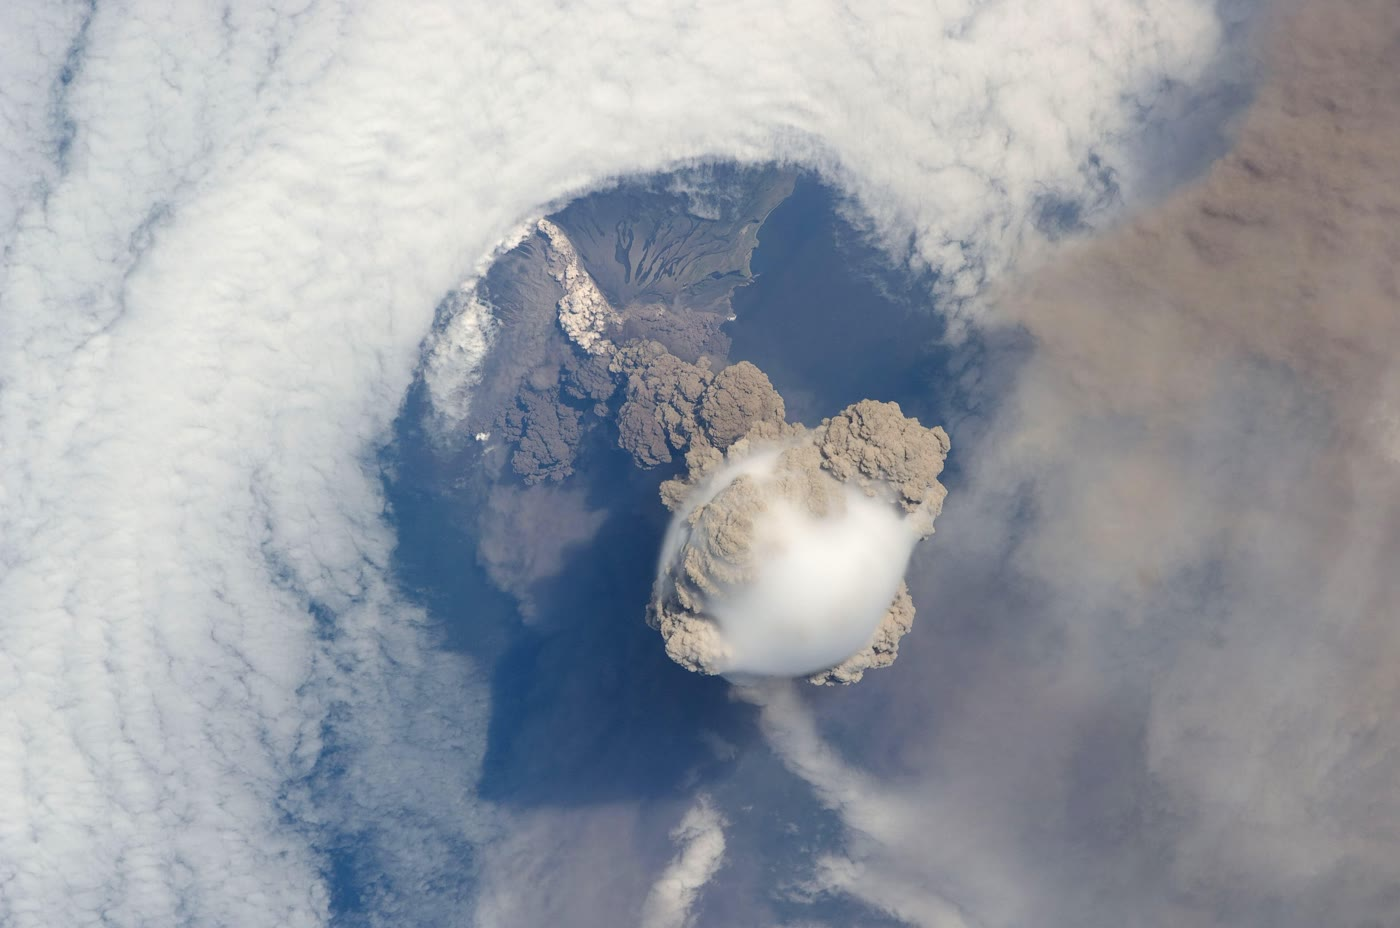
\includegraphics[width=0.66\linewidth]{images/book3/b1-sarychev-iss.jpg}
\par\smallskip{\small Sarychev Peak, gunung api busur Kuril di Pulau Matua, dalam tahap awal erupsi pada 12 Juni 2009, dilihat dari Stasiun Luar Angkasa Internasional melalui celah di awan. Abu kelabu, mungkin aliran piroklastik, mengalir turun dari puncak, dan selubung awan halus, sebuah pileus, duduk di atas kolom yang naik; abu dari erupsi itu terdeteksi lebih dari \qty{2400}{km} jauhnya. Foto: NASA, domain publik (Wikimedia
Commons).}
\label{fig:b1:active-margins:sarychev}
\end{omfigure}
% ledger: nasa:sarychev, commons:sarychev

\omterm{def:b1:layered-earth:layers}{Kerak} di bawah busur menebal baik oleh pemendekan maupun oleh magma yang ditambahkan dari bawah; di bawah busur yang dibangun di atas benua, seperti Andes, ia termasuk yang paling tebal di Bumi.

Di belakang sebagian busur, lempeng yang menindih teregang. Dan Karig menjelaskan cekungan marginal ini di Pasifik barat dalam tektonik lempeng, pada 1971: ketika slab menunjam curam dan menggelinding ke belakang, palung dan busur bermigrasi ke arah lempeng yang menunjam, dan lempeng di belakangnya teregang hingga terbelah, kadang meninggalkan busur sisa yang punah di sisi jauh. Dalam model lempeng yang dipakai di atas, penyebaran busur-belakang berjalan sekitar \qty{32}{mm.yr^{-1}} di Mariana Trough dekat \ang{18}\,LU, dan lebih dari \qty{110}{mm.yr^{-1}} di bagian utara Lau Basin, di belakang Tonga. Sebaliknya, di tempat slab dangkal, ia menarik lempeng yang menindih, yang \omterm{def:b1:layered-earth:layers}{kerak} di belakang busurnya memendek dan menebal, seperti di belakang Andes.
% ledger: karig:marginal-basins, data:pb2002 (ridge_budget.py: Mariana 32.4, Lau 117.5 mm/yr)

\begin{inthefield}[Peringatan tsunami]
Pusat peringatan tsunami hanya punya beberapa menit. Pada 2011 peringatan pertama untuk pantai timur laut Jepang datang sekitar tiga menit setelah gempa bumi, dari suatu magnitudo yang didasarkan pada gelombang seismik periode pendek; untuk gempa bumi bermagnitudo 8 atau lebih, magnitudo seperti itu diremehkan, dan demikian pula tinggi tsunaminya. Magnitudo momen, yang tidak mengalami saturasi, memerlukan sekitar lima belas menit: seismometer pita lebar Jepang telah didorong melampaui jangkauannya. Sejak 2013, ketika besar gempa bumi sebesar itu tidak pasti, peringatan pertama mengandaikan gempa bumi terbesar yang mungkin di sana dan menggambarkan tsunami dengan kata-kata, seperti ``sangat besar'', alih-alih dengan angka; dan prakiraannya bertumpu pada pengukuran laut lepas pantai, dari pelampung yang diposisikan oleh satelit dan pengukur tekanan di dasar laut, yang melihat gelombang sebelum ia mencapai pantai.
% ledger: jma:warning

\smallskip
\begin{center}
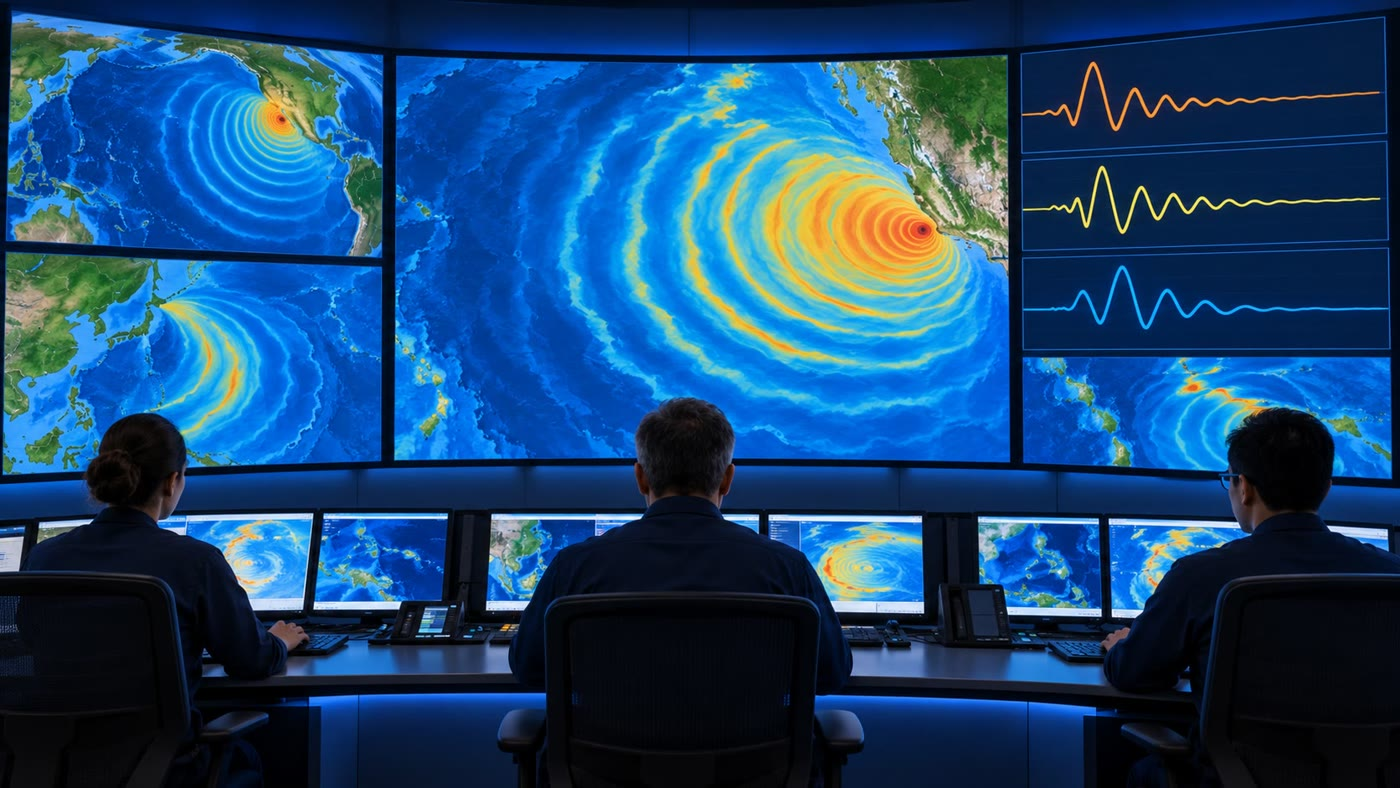
\includegraphics[width=0.7\linewidth]{images/book3/ai/b1-tsunami-centre.jpg}

{\scriptsize Petugas jaga di pusat peringatan tsunami, di depan layar muka gelombang hasil hitungan dan rekaman muka laut (ilustrasi hasil AI).}
\end{center}
\end{inthefield}

\section{Latihan}

\begin{exercise}[$\star$]\label{exo:b1:active-margins:1}
Sebuah palung terletak \qty{3}{km} di bawah dasar samudra di sekitarnya. (a) Jika ia tidak terkompensasi, dengan berapa gravitasi di sana akan berkurang oleh batuan yang hilang, bermassa jenis \qty{2700}{kg.m^{-3}}, yang digantikan oleh air laut bermassa jenis \qty{1000}{kg.m^{-3}}? Gunakan slab Bouguer, dengan $G = \qty{6.674e-11}{m^3.kg^{-1}.s^{-2}}$. (b) Bandingkan dengan anomali yang teramati di atas Palung Kuril, sekitar \qty{-260}{\milli\gal}, tempat palung terletak \qty{3.5}{km} di bawah dasar di sekitarnya: hitung ulang untuk kedalaman itu. (c) Mengapa air di palung yang lebarnya hanya puluhan kilometer memberi hasil yang lebih kecil daripada rumus slab, dan di mana sisa defisitnya harus berada?
\end{exercise}

\begin{exercise}[$\star$]\label{exo:b1:active-margins:2}
Lempeng Pasifik masuk ke Palung Kuril pada \qty{82}{mm.yr^{-1}}. (a) Berapa panjang lempeng yang tenggelam dalam 10 juta tahun? (b) Jika slab tenggelam sepanjang lintasan lurus yang miring \ang{45}, berapa dalam ujung depannya kemudian? (c) Berapa lama waktu yang diperlukan untuk mencapai \qty{600}{km}?
\end{exercise}

\begin{exercise}[$\star$]\label{exo:b1:active-margins:3}
Gunung api berdiri di atas tempat slab lurus berada pada kedalaman \qty{110}{km}. Hitung \omterm{def:b1:active-margins:volcanic-arc}{celah busur--palung} untuk slab yang miring \ang{30}, \ang{45} dan \ang{60}. Busur mana yang paling jauh dari palungnya?
\end{exercise}

\begin{exercise}[$\star$]\label{exo:b1:active-margins:4}
Dalam model lempeng digital bab ini, sekitar \qty{2.7}{km^2} dasar samudra menunjam di sepanjang batas subduksi setiap tahun, sepanjang sekitar \qty{51000}{km}, dan sekitar \qty{3.0}{km^2} dibuat sepanjang sekitar \qty{67000}{km} punggungan penyebaran. (a) Hitung laju konvergensi rata-rata dan \omterm{def:b1:plate-kinematics:spreading-rate}{laju penyebaran penuh} rata-rata, dalam \unit{mm.yr^{-1}}. (b) Di seluruh batasnya model menghancurkan luas sebanyak yang dibuatnya. Ke mana sisa dasar baru itu pergi?
% ledger: data:pb2002 (ridge_budget.py: 2.739 km2 over 51471 km; 3.009 km2 over 67340 km; all 3.511 vs 3.519)
\end{exercise}

\begin{exercise}[$\star\star$]\label{exo:b1:active-margins:5}
Empat gempa bumi pada suatu penampang berada di $(x, z) = (200, 150)$, $(300, 250)$, $(400, 330)$ dan $(500, 430)$, dalam kilometer. (a) Cocokkan garis slab dengan kuadrat terkecil dan berikan \omterm{def:b1:geological-maps:attitude}{kemiringannya}. (b) Di mana garis itu mencapai permukaan? (c) Bandingkan dengan \omterm{def:b1:geological-maps:attitude}{kemiringan} garis yang melalui gempa pertama dan terakhir saja.
\end{exercise}

\begin{exercise}[$\star\star$]\label{exo:b1:active-margins:6}
Sebuah slab model miring \ang{25} dari palung hingga \qty{50}{km}, lalu \ang{45}. Garis depan gunung api berdiri di tempat slab berada pada kedalaman \qty{110}{km}. (a) Hitung \omterm{def:b1:active-margins:volcanic-arc}{celah busur--palung}. (b) Bandingkan dengan slab yang miring \ang{45} sepanjang jalannya. (c) Segmen dalam, jika diperpanjang ke atas, mencapai permukaan: di mana? Bandingkan dengan garis Kuril, yang mencapainya \qty{53}{km} di sisi daratan dari palung. (d) Celah apa yang akan diberikan oleh segmen dalam yang miring \ang{60}?
\end{exercise}

\begin{exercise}[$\star\star$]\label{exo:b1:active-margins:7}
(a) Menurut proposisi kulit bola yang dibengkokkan, berapa jari-jari sudut, dan berapa jari-jari dalam kilometer ($R = \qty{6371}{km}$), yang seharusnya dimiliki sebuah busur di atas slab yang miring \ang{45}? \ang{30}? \ang{70}? (b) Busur mana yang paling ketat melengkung? (c) Slab Kuril miring \ang{44.9} dan Palung Kuril cocok dengan lingkaran \ang{21.9}: hitung selisih relatifnya terhadap prediksi.
\end{exercise}

\begin{exercise}[$\star\star$]\label{exo:b1:active-margins:8}
Ambil konduktivitas \qty{2.5}{W.m^{-1}.K^{-1}} dan suhu permukaan \qty{10}{\celsius}. (a) Hitung gradien suhu permukaan di bawah \omterm{def:b1:active-margins:active-margin}{forearc} yang kehilangan \qty{35}{mW.m^{-2}} dan di bawah \omterm{def:b1:active-margins:active-margin}{cekungan busur-belakang} yang kehilangan \qty{80}{mW.m^{-2}}. (b) Dengan mengekstrapolasi gradien ini secara linear, perkirakan suhu pada \qty{30}{km} di masing-masing. (c) \omterm{def:b1:layered-earth:discontinuity}{Moho} busur-belakang diukur pada 800 hingga \qty{900}{\celsius}. Mengapa perkiraan linear terlalu tinggi?
% ledger: hyndman:backarc (back-arc 70-85, Moho 800-900); the forearc value is an exercise value
\end{exercise}

\begin{exercise}[$\star\star$]\label{exo:b1:active-margins:9}
Dalam model lempeng bab ini, Mariana Trough membuka dekat \ang{18}\,LU dengan laju penuh sekitar \qty{32}{mm.yr^{-1}}. (a) Nyatakan laju ini dalam \unit{km.Ma^{-1}}, dan berikan setengah laju jika penyebarannya simetris. (b) Berapa lama waktu yang diperlukan palung itu untuk membuka sebesar \qty{100}{km} dengan laju ini? (c) Berikan dua alasan mengapa umur \omterm{def:b1:active-margins:active-margin}{cekungan busur-belakang} tidak dapat begitu saja dibaca dari lebarnya dan laju sekarangnya.
% ledger: data:pb2002 (ridge_budget.py: mariana_18n_mm_yr 32.4)
\end{exercise}

\begin{exercise}[$\star\star\star$]\label{exo:b1:active-margins:10}
Sebuah slab setebal \qty{100}{km} menunjam pada \qty{82}{mm.yr^{-1}} sepanjang lintasan yang miring \ang{45}. Ambil $\kappa = \qty{e-6}{m^2.s^{-1}}$. (a) Berapa lama waktu yang diperlukan untuk mencapai \qty{600}{km}? (b) Seberapa jauh panas berdifusi ke dalamnya dalam waktu itu, menurut $\sqrt{\kappa t}$? (c) Berapa lama panas memerlukan waktu untuk mencapai tengahnya? (d) Simpulkan tentang suhu slab pada \qty{600}{km} dan tentang gempa buminya.
\end{exercise}

\begin{exercise}[$\star\star\star$]\label{exo:b1:active-margins:11}
Sebuah \omterm{def:b1:active-margins:accretionary}{prisma akresi} model memiliki penampang segitiga: permukaannya miring $\alpha = \ang{4}$ ke arah palung dan dasarnya miring $\beta = \ang{6}$ di bawahnya, keduanya bertemu di ujungnya; ia mempertahankan sudut-sudut ini saat tumbuh. (a) Tunjukkan bahwa luasnya adalah $A = \frac12 L^2(\tan\alpha + \tan\beta)$ untuk lebar $L$, ketika sudut-sudutnya cukup kecil sehingga tinggi di bagian belakang adalah $L(\tan\alpha + \tan\beta)$. (b) Sedimen setebal \qty{1}{km} tiba di lempeng yang konvergen pada \qty{40}{mm.yr^{-1}}, dan semuanya terakresi: hitung lebar setelah 1, 4 dan 10 juta tahun. Bagaimana $L$ tumbuh terhadap waktu? (c) Bagaimana jika separuh sedimennya ikut turun bersama slab?
\end{exercise}

\begin{exercise}[$\star\star\star$]\label{exo:b1:active-margins:12}
(a) Tunjukkan bahwa garis kuadrat terkecil melalui titik rata-rata $(\bar x, \bar z)$. (b) Sebuah katalog mendaftarkan setiap kedalaman \qty{10}{km} terlalu dalam. Bagaimana \omterm{def:b1:geological-maps:attitude}{kemiringan} dan perpotongan garis yang dicocokkan berubah? (c) Jarak $x$ semuanya diukur dari titik palung yang ditempatkan \qty{20}{km} terlalu jauh ke arah daratan, sehingga setiap $x$ \qty{20}{km} terlalu kecil. Bagaimana \omterm{def:b1:geological-maps:attitude}{kemiringan} dan perpotongan berubah? (d) Apakah kesalahan mana pun mengubah \omterm{def:b1:geological-maps:attitude}{kemiringannya}?
\end{exercise}

\section{Masalah: membaca zona subduksi dari gempanya}

\begin{problem}[{Soal akhir pekan --- slab Kuril dari delapan gempa bumi, seberapa cepat ia tenggelam, apa yang dikatakan gravitasi dan aliran panasnya, dan di mana gunung apinya seharusnya berdiri}]
\label{pb:b1:active-margins:1}
% nilai: calc/ch14.py; kedelapan peristiwa itu nyata (katalog USGS, dibulatkan ke kilometer)
% dari figdata/out/bachelor-1-slab_seismicity-section.dat
% ledger: data:b3-usgs-kuril, data:pb2002, data:b2-seafloor-age, syracuse:arc-depth, frank:arcs,
% data:b3-grav-kuril, parsons:plate-model, hyndman:backarc; aliran panas forearc adalah nilai latihan
Delapan gempa bumi slab Kuril, semuanya lebih dalam dari \qty{70}{km}, didaftar menurut jaraknya $x$ dari palung sepanjang garis penampang, ke arah Laut Okhotsk, dan kedalamannya $z$, keduanya dibulatkan ke kilometer.

\begin{center}
\small
\begin{tabular}{lcccccccc}
\hline
peristiwa & 1 & 2 & 3 & 4 & 5 & 6 & 7 & 8\\
$x$ (\unit{km}) & 155 & 222 & 305 & 319 & 431 & 533 & 578 & 609\\
$z$ (\unit{km}) & 96 & 169 & 245 & 272 & 389 & 489 & 518 & 573\\
magnitudo & 5.5 & 5.1 & 5.0 & 5.4 & 5.3 & 5.3 & 5.2 & 6.4\\
\hline
\end{tabular}
\end{center}

\medskip
\noindent\textbf{Bagian I --- Garis slab.}
\begin{enumerate}
  \item Gambarkan kedelapan gempa bumi dalam skala yang sama pada kedua sumbu, dengan
        kedalaman ke bawah.
  \item Hitung $\sum x_i$, $\sum z_i$, $\sum x_i^2$, $\sum x_i z_i$ dan rata-rata
        $\bar x$ dan $\bar z$.
  \item Hitung $S_{xx}$ dan $S_{xz}$, lalu \omterm{def:b1:geological-maps:attitude}{kemiringan} garis kuadrat terkecil hingga tiga
        desimal dan perpotongannya hingga satu desimal.
  \item Berapa \omterm{def:b1:geological-maps:attitude}{kemiringan} slab?
  \item Di mana garis itu mencapai permukaan? Apa yang dikatakan ini tentang bentuk slab
        di dekat palung?
  \item Hitung simpangan $z_i - (a + s x_i)$ tiap gempa bumi. Yang manakah paling jauh dari
        garis, dan berapa jaraknya?
\end{enumerate}

\medskip
\noindent\textbf{Bagian II --- Seberapa cepat slab tenggelam.} Pada awal penampang model
PB2002 memberikan konvergensi sebesar \qty{87.4}{mm.yr^{-1}}: relatif terhadap Lempeng
Okhotsk, Lempeng Pasifik bergerak ke arah \omterm{def:b1:spherical-astronomy:horizontal}{azimut} \ang{300}. Garis penampang, tegak lurus
terhadap palung, berjalan ke arah \omterm{def:b1:spherical-astronomy:horizontal}{azimut} \ang{320.9}.
\begin{enumerate}[resume]
  \item Hitung sudut antara konvergensi dan garis penampang, lalu komponen konvergensi yang
        tegak lurus dan sejajar dengan palung.
  \item Berapa panjang lempeng yang tenggelam ke palung dalam 10 juta tahun?
  \item Dengan menggunakan \omterm{def:b1:geological-maps:attitude}{kemiringan} pada soal 4 (dibulatkan menjadi \ang{45}), berapa lama
        slab memerlukan waktu untuk membawa sebuah titik dari puncaknya, dari palung hingga ke
        gempa bumi terdalam pada pita itu, \qty{632}{km}? Abaikan \omterm{def:b1:geological-maps:attitude}{kemiringan} yang lebih landai di
        dekat palung.
  \item Lempeng itu berumur sekitar \qty{122}{Ma} di palung. Berapa umur dasar laut yang kini
        terletak pada kedalaman \qty{632}{km}?
  \item Dengan $\sqrt{\kappa t}$, dengan $\kappa = \qty{e-6}{m^2.s^{-1}}$, seberapa jauh panas
        telah berdifusi ke dalam slab selama turunan itu? Bandingkan dengan tebalnya, sekitar
        \qty{100}{km}.
\end{enumerate}

\medskip
\noindent\textbf{Bagian III --- Gravitasi dan aliran panas.} Ambil konduktivitas
\qty{2.5}{W.m^{-1}.K^{-1}}.
\begin{enumerate}[resume]
  \item Dasar samudra tua di depan palung kehilangan sekitar \qty{43}{mW.m^{-2}}, busur-belakang
        sekitar \qty{80}{mW.m^{-2}}; ambil \qty{35}{mW.m^{-2}} untuk \omterm{def:b1:active-margins:active-margin}{forearc}. Hitung gradien suhu
        dekat permukaan masing-masing.
  \item Jelaskan mengapa \omterm{def:b1:active-margins:active-margin}{forearc} kehilangan lebih sedikit panas daripada dasar samudra tua di
        depannya.
  \item \omterm{def:b1:isostasy-gravity:anomalies}{Anomali udara-bebas} di atas Palung Kuril sekitar \qty{-260}{\milli\gal}. Berapa tebal
        batuan, \qty{1700}{kg.m^{-3}} lebih padat daripada air, yang dibutuhkan slab Bouguer untuk
        memberikan defisit ini? Bandingkan dengan kedalaman palung di bawah dasar di sekitarnya,
        sekitar \qty{3.5}{km}.
  \item Anggap sekarang seluruh lempeng didorong ke bawah sebesar \qty{3.5}{km}: air menggantikan
        batuan di bagian atasnya, dan \omterm{def:b1:layered-earth:layers}{keraknya} menggantikan \omterm{def:b1:layered-earth:layers}{mantel} di dasarnya, sehingga, secara
        keseluruhan, \omterm{def:b1:layered-earth:layers}{mantel} bermassa jenis \qty{3300}{kg.m^{-3}} digantikan oleh air. Hitung anomali slab
        Bouguer. Mengapa palung yang sebenarnya, yang lebarnya hanya puluhan kilometer, memberi
        lebih kecil?
  \item Palung dan tonjolan luar tidak berada dalam kesetimbangan isostatik. Apa yang menahan
        keduanya di luar kesetimbangan itu?
\end{enumerate}

\medskip
\noindent\textbf{Bagian IV --- Di mana gunung api seharusnya berdiri.} Gunakan garis dari soal 3,
dengan \omterm{def:b1:geological-maps:attitude}{kemiringan} dan perpotongannya yang dibulatkan.
\begin{enumerate}[resume]
  \item Gunung api pertama dalam pita itu berjarak \qty{164}{km} dari palung. Berapa dalam slab di
        bawahnya?
  \item Apakah kedalaman ini berada dalam rentang yang ditemukan di bawah busur, 72 hingga
        \qty{173}{km}? Berapa jauhnya dari rata-rata, \qty{105}{km}?
  \item Pada jarak berapa dari palung slab berada pada kedalaman \qty{100}{km}?
  \item Menurut proposisi kulit bola yang dibengkokkan, berapa jari-jari sudut yang seharusnya
        dimiliki busur Kuril, dan berapa jari-jarinya dalam kilometer?
  \item Palung Kuril cocok dengan \omterm{def:b1:spherical-astronomy:spherical-triangle}{lingkaran kecil} \ang{21.9}. Bandingkan.
  \item \omterm{def:b1:active-margins:volcanic-arc}{Busur gunung api} berdiri, rata-rata, di tempat slab berada pada kedalaman sekitar
        \qty{105}{km}. Pada jarak berapa dari palung garis slab mencapai kedalaman itu?
  \item Bandingkan jarak ini dengan \qty{164}{km} yang teramati: dengan berapa kilometer dan
        dengan pecahan berapa ia berbeda?
  \item Hingga kilometer terdekat, \omterm{def:b1:active-margins:volcanic-arc}{celah busur--palung} apa yang diprediksi garis slab Kuril untuk
        gunung api yang berdiri di atas slab pada \qty{105}{km}?
\end{enumerate}
\end{problem}
